\chapter{Laplacetransformatie}
\section{De Heaviside functie}
De Heaviside functie heeft als voorschrift:
$$H(t - a) = 
\begin{cases}
0 \;\; t < a \\
1 \;\; t > a
\end{cases}$$

\example{Teken over $x=[-3,4]$ de functie $y = 2H(t + 2) - tH(t) + (t+t^2)H(t-2)$}
{
Er zijn veranderingen bij $t = -2, t = 0$ en $t = 2$.

    \begin{tabular}{l | l}
    $2\cdot(0) - t\cdot(0) + (t+t^2)\cdot(0) = 0$ & $t < -2$\\
    $2\cdot(1) - t\cdot(0) + (t+t^2)\cdot(0) = 2$ & $-2 < t < 0$  \\
    $2\cdot(1) - t\cdot(1) + (t+t^2)\cdot(0) = 2 - t$ & $0 < t < 2$\\
    $2\cdot(1) - t\cdot(1) + (t+t^2)\cdot(1) = 2 + t^2$ & $t > 2$\\
    \end{tabular}
\todo{graph}
}
\example{Schrijf met behulp van de Heaviside functie de stuksgewijze continue functie:
$$f(t) = \begin{cases}
        e^t & t < 2 \\
        1 - e^t & 2 < t < 3 \\
        t^2 & 3 < t < 5 \\
        t - 25 & t > 5
        \end{cases}
$$}{
\begin{equation*}
\begin{split}
    f(t) & = e^t + H(t-2)(-e^t + 1 - e^t) + H(t-3)(-1 + e^t + t^2) + H(t - 5)(-t^2 + t - 25) \\
    & = e^t + (1-2e^t)H(t-2) + (t^2+e^t-1)H(t-3) - (t^2-t+25)H(t-5)
\end{split}
\end{equation*}
}

\section{De Dirac delta-'functie'}
De Dirac delta-functie heeft als voorschrift:
$$
\begin{cases}
\delta(t - a) = 0 & t \neq a \\
\int_{a - \epsilon_1}^{a + \epsilon_2} \delta(t - a) \; dt = 1 & \forall \epsilon_1, \epsilon_2 > 0 
\end{cases}
$$
De meetkundige betekenis: We nemen de limiet van $\delta^a_{\epsilon_1,\epsilon_2}(t)$ voor $\epsilon_1,\epsilon_2 \rightarrow 0$
$$\delta^a_{\epsilon_1,\epsilon_2}(t) = \begin{cases}
                                        0 & \forall t < a - \epsilon_1 \; \hbox{of} \; t > a + \epsilon_2 \\
                                        \frac{1}{\epsilon_1 + \epsilon_2} & \forall \in ]a - \epsilon_1, a + \epsilon_2[
                                        \end{cases}
$$
Het nut van de dirac functie is om bepaalde integralen op te lossen. Meer bepaald de integralen van de vorm:
$$\int_{0}^{+\infty} f(t) \delta(t- a)\;dt = f(a)$$
De ondergrens 0 mag ook vervangen worden door $-\infty$ aangezien elke functie causaal is binnen het domein van Laplace.

De afgeleide van de Heaveiside functie is gelijk aan de delta functie:
$$\frac{d}{dt}H(t-a) = \delta(t - a)$$
\example{$$\int_{0}^{+\infty} (2\sin t - 1) \delta(t - \frac{3\pi}{2}) \; dt$$}{
In dit geval is $f(t) = (2\sin t - 1)$ en $\delta(t - a) = \delta(t - \frac{3\pi}{2})$
We kunnen dus makkelijk deze integraal oplossen door gebruik te maken van de definitie:
\begin{equation*}
\begin{split}
\int_{0}^{+\infty} f(t) \delta(t- a)\;dt & = \int_{0}^{+\infty} (2\sin t - 1) \delta(t - \frac{3\pi}{2}) \; dt \\
                                        & = f(\frac{3\pi}{2}) - 1  \\
                                        & = 2\sin \bigg(\frac{3\pi}{2}\bigg) - 1 \\
                                        & = -2 - 1 \\
                                        & = - 3
\end{split}
\end{equation*}
}
\section{Causale functie}
Een causale functie is een functie $f$ waarvoor $f(t) = 0$ voor elke $t < 0$.
Om een willekeurige functie causaal te maken voeg je de Heaviside functie achteraan toe.
$$f(t) \rightarrow f(t)H(t)$$
Dit zorgt ervoor dat voor elke $t < 0$ dat $f(t) = 0$. De afspraak is dat deze Heaviside functie nu achter elke functie komt zonder dat we deze nog schrijven. Elke functie is vanaf nu dus causaal.

\example{Teken de causale functie $f(t)$ gedefinieerd als: -2 indien t $<$ 1 en 2 als t $>$ 1. Schrijf ze ook met behulp van de Heaviside functie}{
De functie kan omschreven worden als:
$$f(t) = \begin{cases}
        0 & t < 0 \\
        -2 & 0 < t < 1 \\
        2 & t > 1
        \end{cases}
$$
Omgevormd met de Heaviside-functie:
\begin{equation*}
\begin{split}
f(t) & = H(t)(-0 + (-2)) + H(t -  1)(-2 +2) \\
    & = -2H(t) + 4H(t - 1)
\end{split}
\end{equation*}
Tekening:

\begin{center}
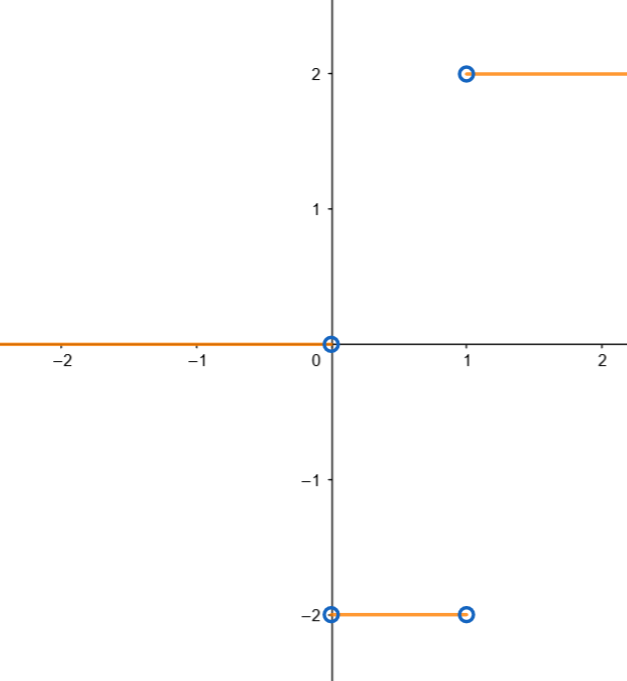
\includegraphics[width=0.8\textwidth]{oef5_heaviside}
\end{center}
}
\section{Exponentiële orde}
Een functie is van exponentiële orde indien $\exists M, a \in R$ zodat $|f(t)| < Me^{at}, \forall t > N$ en met a het minimum van de waarden waarvoor dit geldt. Indien waar is $f(t)$ van exponentiële orde a.
Soms is het gemakkelijker te bewijzen via:
$$\lim_{t \to +\infty} \frac{|f(t)|}{e^{at}} \in R$$
\example{Bepaal de exponentiële orde van $\sin t$}{
\begin{equation*}
\begin{split}
                & |\sin t| \leq 1 \\
\Leftrightarrow & |\sin t| < 1.1 \hbox{(willekeurige waarde)} \\
\Leftrightarrow & |\sin t| < 1.1e^{at}
\end{split}
\end{equation*}
Hieruit kan afgeleid worden dat a = 0 en de exponentiële orde is dus ook 0.
}
\example{Bepaal de exponentiële orde van $(1 + 2t)e^{-t}$}{
Bij deze opgave maken we gebruik van de limietstelling.
\begin{equation*}
\begin{split}
\lim_{t \to +\infty} \frac{|f(t)|}{e^{at}} & = \lim_{t \to +\infty} \frac{|(1 + 2t)e^{-t}|}{e^{at}} \\
                                            & = \lim_{t \to +\infty} \frac{(1 + 2t)e^{-t}}{e^{at}} \\
                                            & = \lim_{t \to +\infty} \frac{1 + 2t}{e^{at}e^{t}} \\
                                            & = \lim_{t \to +\infty} \frac{1 + 2t}{e^{t(a +1)}} 
\end{split}
\end{equation*}
We moeten een onderscheid maak tussen 2 gevallen:
\begin{itemize}
\item $a + 1 < 0 \rightarrow e^{-\infty} = 0 \rightarrow \frac{+\infty}{0} \rightarrow \; \hbox{onbepaald}$
\item $a + 1 > 0 \rightarrow e^{+\infty} = \infty \rightarrow \frac{+\infty}{+\infty} \rightarrow \; \hbox{L'Hopital}$
\end{itemize}
We maken enkel gebruik van het tweede geval en passen dus L'hopital toe.
\begin{equation*}
\begin{split}
\lim_{t \to +\infty} \frac{1 + 2t}{e^{t(a +1)}} & = \lim_{t \to +\infty} \frac{2}{e^{t(a +1)}(a+1)} \\
                                                & = \frac{2}{+\infty} = 0 \in R
\end{split}
\end{equation*}
Aangezien het een reëele uitkomst is kan a uit de uitdrukking $a + 1 > 0$ afgeleid worden.
$$\forall a, a > -1$$
De exponentiële orde is dus -1.
}
\section{De Laplacetransformatie}
Definitie: Stel $f(t)$ causuaal dan is de laplacetransformatie van $f(t)$ een functie die een complex getal $s$ afbeeldt op 
$$\mathcal{L}\{f(t)\}(s) = F(s) = \int_{0}^{+\infty}f(t)e^{-st}\;dt, s \in \mathbb{C}$$
Een voorbeeld uit het formularium:
$$\mathcal{L}\{\sin t\}(s) = \frac{1}{1 + s^2}$$
De letter s kan eender welk complex getal zijn:
$$\mathcal{L}\{\sin t\}(2) = \frac{1}{1 + 4}$$
Indien er een imaginaire eenheid is verandert de definitie minimaal:
$$\mathcal{L}\{\sin t\}(3 + 2j) = \int_{0}^{+\infty}|f(t)e^{-st}|\;dt$$
Het argument tussen de $| ... |$ is NIET de absolute waarde, maar de MODULUS van het complexe getal, te berekenen via $\sqrt{x^2 + y^2}$ indien het complexe getal gedefinieerd wordt als $s = x + yj$ (wat vanaf nu als definitie gebruikt wordt voor een complex getal).
\subsection{Opmerkingen}
\begin{enumerate}
\item $$|f(t)e^{-st}| = |f(t)|e^{-xt}, \; s = x+yj$$
want
\begin{equation*}
\begin{split}
|f(t)e^{-st}| & = |f(t)e^{-(x + yj)t}| \\
                & = |f(t)|\cdot|e^{-(xt + yjt)}| \\
                & = |f(t)|\cdot|e^{-xt} \cdot e^{-yjt}| \\
                & = |f(t)|\cdot|e^{-xt}|\cdot|e^{-yjt}| \\
                & = |f(t)|\cdot e^{-xt}\cdot|\cos(-yt) + j\sin(-yt)| \\
                & = |f(t)|e^{-xt}\sqrt{\cos^2{(-yt)} + \sin^2{(-yt)}} \\
                & = |f(t)|e^{-xt}
\end{split}
\end{equation*}
\item 
$$\mathcal{L}\{af(t) + bg(t)\}(s) = a\mathcal{L}\{f(t)\}(s) + b\mathcal{L}\{g(t)\}(s)$$
De Laplace van een som is gelijk aan de som van een Laplace.
\end{enumerate}
\subsection{Laplacegetransformeerde van enkele basisfuncties}
\begin{itemize}
\item $$\mathcal{L}\{e^{at}\}(s) = \frac{1}{s - a}$$
Bewijs:
\begin{equation*}
\begin{split}
\mathcal{L}\{e^{at}\}(s) & = \int_{0}^{+\infty}e^{at}e^{-st} \; dt \\
                            & = \int_{0}^{+\infty} e^{t(a - s)} \; dt \\
                            & = \frac{e^t{a - s)}}{a - s}\bigg|_{0}^{+\infty} \\
                            & = \frac{1}{a - s}\bigg(\lim_{t \to +\infty}e^{t(a - s)} - 1\bigg)                         
\end{split}
\end{equation*}
Uitwerking van de limiet:
\begin{equation*}
\begin{split}
    \lim_{t \to +\infty}e^{t(a - s)} & = \lim_{t \to +\infty}|e^{at - st)} | \\
                                    & = \lim_{t \to +\infty}|e^{at - (x + yj)t}| \\
                                    & = \lim_{t \to +\infty}|e^{at - xt}\cdot e^{-yjt}| \\
                                    & = \lim_{t \to +\infty}|e^{at - xt}|\cdot |e^{-yjt}| \\
                                    & = \lim_{t \to +\infty}|e^{at - xt}|\cdot |\cos(-yt) + j\sin(-yt)| \\
                                    & = \lim_{t \to +\infty}e^{at - xt}\cdot \sqrt{\cos^2(-yt) + \sin^2(-yt)} \\
                                    & = \lim_{t \to +\infty}e^{at - xt} = e^{-\infty} = 0
\end{split}
\end{equation*}
Deze uitkomst in de oorspronkelijke vergelijking steken:
$$\frac{1}{a - s}(0 - 1) = \frac{1}{s - a}$$ 

\item $$\mathcal{L}\{\sin \omega t\}(s) = \frac{\omega}{\omega^2 + s^2} \qquad  \hbox{en} \qquad  \mathcal{L}\{\cos \omega t\}(s) = \frac{s}{\omega^2 + s^2}$$
Bewijs: We vertrekken van de uitkomst van vorig bewijs. Beschouw $a = wj$
\begin{equation*}
\begin{split}
\mathcal{L}\{e^{wjt}\}(s) & = \frac{1}{s - wj} \\
                            & = \frac{1}{s - wj} \cdot \frac{s + wj}{s + wj} \\
                & = \frac{s + wj}{s^2 + w^2}\\
                & = \mathcal{L}\{\cos (\omega t) + j\sin(\omega t)\}(s) \\
                & = \mathcal{L}\{\cos (\omega t)\}(s) + \mathcal{L}\{j\sin(\omega t) \}(s) \\
                & = \frac{s}{s^2 + w^2} + \frac{w}{s^2 + w^2}j \\ 
\end{split}
\end{equation*}
dus $$\mathcal{L}\{\cos \omega t\}(s) = \frac{s}{\omega^2 + s^2} \qquad  \hbox{en} \qquad  \mathcal{L}\{\sin \omega t\}(s) = \frac{\omega}{\omega^2 + s^2}$$

\item 
$$\mathcal{L}\{\delta(t)\}(s) = 1$$
Bewijs:
\begin{equation*}
\begin{split}
    \mathcal{L}\{\delta(t)\}(s) & = \mathcal{L}\{\delta(t - 0)\}(s) \\
                & = \int_{0}^{+\infty}\delta(t - 0)e^{-st}\;dt \\
                & = f(0) = e^{-s\cdot0} = e^{0} = 1
\end{split}
\end{equation*}
\end{itemize}
\example{Bepaal het laplacebeeld van $\cos{(2t - 1)}$}{
\begin{equation*}
\begin{split}
\mathcal{L}\{\cos(2t - 1)\}(s) & = \mathcal{L}\{\cos(2t)\cos( 1 )+ \sin(2t)\sin (1)\}(s) \\
                & = \cos (1) \mathcal{L}\{\cos 2t\}(s) + \sin (1 )\mathcal{L}\{\sin 2t\}(s)\\
                & = \cos (1) \frac{s}{s^2 + 4} + \sin (1) \frac{2}{s^2 + 4} \\
                & = \frac{s\cos(1)}{s^2 + 4} + \frac{2\sin(1)}{s^2 + 4}
\end{split}
\end{equation*}
}
\example{Bepaal het laplacebeeld van $\sinh(4t) - 3\cos{(\frac{t}{3})}$}
{
\begin{equation*}
\begin{split}
\mathcal{L}\bigg\{\ \sinh(4t) - 3\cos{\bigg(\frac{t}{3}\bigg)} \bigg\}(s) & = \mathcal{L}\bigg\{\ \frac{e^{4t} - e^{-4t}}{2} - 3\cos{\bigg(\frac{t}{3}\bigg)} \bigg\}(s) \\
& = \mathcal{L}\bigg\{\ \frac{e^{4t} - e^{-4t}}{2}\bigg\}(s) - 3\mathcal{L}\bigg\{\cos{\bigg(\frac{t}{3}\bigg)} \bigg\}(s) \\
& = \frac{1}{2}\bigg(\frac{1}{s - 4} - \frac{1}{s + 4}\bigg) - 3\frac{s}{s^2 + \frac{1}{9}} \\
& = \frac{1}{2}\bigg(\frac{1}{s - 4} - \frac{1}{s + 4}\bigg) - \frac{27s}{9s^2 + 1}
\end{split}
\end{equation*}
}
\example{Bepaal het laplacebeeld van $\delta(t - \frac{\pi}{2})\cos(4t)e^{2t}$}{
\begin{equation*}
\begin{split}
\mathcal{L}\bigg\{\delta\bigg(t - \frac{\pi}{2}\bigg)\cos(4t)e^{2t}\bigg\}(s) & = \int_{0}^{+\infty}\cos(4t)e^{2t}\delta\bigg(t - \frac{\pi}{2}\bigg)e^{-st} \; dt \\
& = f\bigg(\frac{\pi}{2}\bigg) \\
& = \cos\bigg(4 \cdot \frac{\pi}{2}\bigg)e^{2\cdot\frac{\pi}{2}}e^{-s\cdot\frac{\pi}{2}} \\
& = \cos(2\pi)e^{\pi}e^{-\frac{s\pi}{2}}\\
& = e^{\pi}e^{-\frac{s\pi}{2}}
\end{split}
\end{equation*}

}
\subsection{Translatie naar rechts}
Definitie:
$$\mathcal{L}\{f(t - a)H(t - a)\}(s) = e^{-as}F(s) \qquad a > 0$$
Bewijs:
\begin{equation*}
\begin{split}
\mathcal{L}\{f(t - a)H(t - a)\}(s) & = \int_{0}^{+\infty}f(t - a)H(t - a)e^{-st} \; dt \\
                                    & = \int_{0}^{a}f(t - a)H(t - a)e^{-st} \; dt + \int_{a}^{+\infty}f(t - a)H(t - a)e^{-st} \; dt \\
                                    & = 0 +\int_{a}^{+\infty}f(t - a)H(t - a)e^{-st} \; dt \\
                                    & = \int_{a}^{+\infty}f(t - a)H(t - a)e^{-st} \; dt \\
                                    \hbox{stel}\quad u & = t - a \\
                                    \hbox{dan}\quad du & = dt \\    
                                    & = \int_{0}^{+\infty}f(u)e^{-s(u + a)} \; du \\
                                    & = \int_{0}^{+\infty}f(u)e^{-su}e^{-sa} \; du \\
                                    & = e^{-sa}\int_{0}^{+\infty}f(u)e^{-su} \; du \\
                                    & = e^{-sa}\mathcal{L}\{f(t)\}(s) \\
                                    & = e^{-as}F(s)
\end{split}
\end{equation*}
\example{Bepaal het laplacebeeld van $f(t) = (t^2 - 1)H(t - 1) - \sin(3t)H(t - \pi)$}
{
\begin{equation*}
\begin{split}
\mathcal{L}\{f(t)\} & = \mathcal{L}\{(t^2 - 1)H(t - 1)\}(s) - \mathcal{L}\{\sin(3t)H(t-\pi)\}(s)
\end{split}
\end{equation*}
We werken beide laplacetransformaties afzonderlijk uit:
\begin{equation*}
\begin{split}
%t^2 - 1 = (t - 1)^2 + 2t - 2 = (t - 1)^2 + 2(t - 1)%
\mathcal{L}\{(t^2 - 1)H(t - 1)\}(s) & = \mathcal{L}\{[(t-1)^2 + 2(t - 1)]H(t - 1)\}(s)\\
                                    & = e^{-as}\mathcal{L}\{t^2 + 2t\}(s) \\
                                    & = e^{-s}\bigg(\frac{2!}{s^3} + 2\frac{1!}{s^2}\bigg) \\
                                    & = e^{-s}\bigg(\frac{2}{s^3} + \frac{2}{s^2}\bigg)\\
                                    & = e^{-s}\bigg(\frac{2(1 + s)}{s^3}\bigg)
\end{split}
\end{equation*}
\begin{equation*}
\begin{split}
    %sin 3t = sin(3(t - \pi)) + 3\pi) = sin(3(t - \pi) + \pi) = -sin(3(t-\pi))%
\mathcal{L}\{\sin(3t)H(t-\pi)\}(s) & =  \mathcal{L}\{-\sin(3(t - \pi))H(t-\pi)\}(s) \\
                                    & = -e^{-\pi s}\mathcal{L}\{\sin (3t)\}(s) \\
                                    & = -e^{-\pi s}\frac{3}{s^2 + 9} \\
                                    & = -\frac{3e^{-\pi s}}{s^2 + 9}
\end{split}
\end{equation*}
Het resultaat wordt:
\begin{equation*}
\begin{split}
\mathcal{L}\{f(t)\} & = \mathcal{L}\{(t^2 - 1)H(t - 1)\}(s) - \mathcal{L}\{\sin(3t)H(t-\pi)\}(s) \\
                    & = e^{-s}\bigg(\frac{2(1 + s)}{s^3}\bigg) - \bigg(-\frac{3e^{-\pi s}}{s^2 + 9}\bigg) \\
                    & = e^{-s}\bigg(\frac{2(1 + s)}{s^3}\bigg) +\frac{3e^{-\pi s}}{s^2 + 9}
\end{split}
\end{equation*}
}
\subsection{Dempingsfunctie}
Definitie:
$$\mathcal{L}\{e^{-at}f(t)\}(s) = F(s + a)$$
\example{Bepaal het laplacebeeld van $f(t) = t(t^3 - 1)^2e^{-t} + \sin(\sqrt{3}t)e^{2t}$}
{
\begin{equation*}
\begin{split}
\mathcal{L}\{f(t)\}(s) = \mathcal{L}\{t(t^3 - 1)^2e^{-t}\}(s) + \mathcal{L}\{\sin(\sqrt{3}t)e^{2t}\}(s)
\end{split}
\end{equation*}
Ook hier beschouwen we beide laplacetransformaties apart.
\begin{equation*}
\begin{split}
\mathcal{L}\{t(t^3 - 1)^2e^{-t}\}(s) & = \mathcal{L}\{(t^7 - 2t^4 + t)e^{-t}\}(s) \\
                                    & = \mathcal{L}\{t^7 - 2t^4 + t\}(s + 1) \\
                                    & = \frac{7!}{(s + 1)^8} - \frac{2 \cdot 4!}{(s + 1)^5} + \frac{1!}{(s + 1)^2} \\
                                    & = \frac{7!}{(s + 1)^8} - \frac{48}{(s + 1)^5} + \frac{1}{s^2 + 2s + 1}
\end{split}
\end{equation*}
\begin{equation*}
\begin{split}
\mathcal{L}\{\sin(\sqrt{3}t)e^{2t}\}(s) & = \mathcal{L}\{\sin(\sqrt{3}t)\}(s - 2) \\
                                        & = \frac{\sqrt{3}}{(s - 2)^2 + 3} \\
                                        & = \frac{\sqrt{3}}{s^2 -2s + 7}
\end{split}
\end{equation*}
Het resultaat wordt:
\begin{equation*}
\begin{split}
\mathcal{L}\{f(t)\}(s) & = \mathcal{L}\{t(t^3 - 1)^2e^{-t}\}(s) + \mathcal{L}\{\sin(\sqrt{3}t)e^{2t}\}(s) \\
                        & = \frac{7!}{(s + 1)^8} - \frac{48}{(s + 1)^5} + \frac{1}{s^2 + 2s + 1} + \frac{\sqrt{3}}{s^2 -2s + 7}
\end{split}
\end{equation*}
}
\subsection{Schaalwijziging}
Definitie:
$$\mathcal{L}\{f(at)\}(s) = \frac{1}{a}F(\frac{s}{a})$$
Bewijs:
\begin{equation*}
 \begin{split}
  \mathcal{L}\{f(at)\}(s) & = \int_{0}^{+\infty}f(at)e^{-st}\;dt \\
                    \hbox{stel}\; u & = at \\
                    \hbox{dan}\; du & = adt \\
                          & =  \int_{0}^{+\infty}f(u)e^{-s\frac{u}{a}}\;\frac{du}{a} \\
                          & =  \frac{1}{a}\int_{0}^{+\infty}f(u)e^{-\frac{s}{a}u}\;du \\
                          & =  \frac{1}{a}\mathcal{L}\{f(u)\}(\frac{s}{a}) \\
                          & =  \frac{1}{a}F(\frac{s}{a})
 \end{split}
\end{equation*}
\example{Gegeven $\mathcal{L}\{\sin t\}(s) = \frac{1}{s^2 + 1}$. Bepaal $\mathcal{L}\{\sin \omega t\}(s)$}
{
\begin{equation*}
 \begin{split}
  \mathcal{L}\{f(\omega t)\}(s) & = \mathcal{L}\{\sin \omega t\}(s) \\
                                & = \frac{1}{\omega}\mathcal{L}\{\sin t\}(\frac{s}{\omega}) \\
                                & = \frac{1}{\omega}\frac{1}{\frac{s^2}{\omega^2} + 1} \\
                                & = \frac{\omega}{\omega^2(\frac{s^2}{w^2} + 1)} \\
                                & = \frac{\omega}{s^2 + w^2}
 \end{split}
\end{equation*}}
\subsection{Laplacegetransformeerde van f'(t)}
Definitie:
$$\mathcal{L}\bigg\{\frac{df(t)}{dt}\bigg\}(s) = sF(s) - f(0^+), \forall s \in \mathbb{C}, Re(s) > a$$
\example{Gegeven $\mathcal{L}\{\sin \omega t\}(s) = \frac{\omega}{s^2 + w^2}$. Bepaal $\mathcal{L}\{\cos\omega t\}(s)$. }{
\begin{equation*}
 \begin{split}
  \mathcal{L}\{\cos\omega t\}(s) & = \mathcal{L}\bigg\{\frac{d[\sin \omega t]}{dt}\bigg\}(s) \\
                                 & = s\mathcal{L}\{\sin \omega t\}(s) - \sin{\omega \cdot 0} \\
                                 & = s\frac{\omega}{s^2 + w^2}
 \end{split}
\end{equation*}
\begin{equation*}
 \begin{split}
                  & \mathcal{L}\{\omega \cos\omega t\}(s) = s\frac{\omega}{s^2 + w^2} \\
  \Leftrightarrow & \omega \mathcal{L}\{\cos\omega t\}(s) = \omega\frac{s}{s^2 + w^2} \\
  \Leftrightarrow & \mathcal{L}\{\cos\omega t\}(s) = \frac{s}{s^2 + w^2} \\
 \end{split}
\end{equation*}}
\subsection{Laplacegetransformeerde van f''(t)}
Definitie:
$$\mathcal{L}\{f^{(n)}(t)\}(s) = s^nF(s) - s^{n - 1}f(0^+) - s^{n -2}f'(0^+) - ... - sf^{(n - 2)}(0^+) - f^{(n-1)}(0^+)$$
\example{Gegeven $g(t) = te^{-t}$, bepaal $\mathcal{L}\{g''(t)\}(s)$}{
\begin{equation*}
 \begin{split}
  \mathcal{L}\{g''(t)\}(s) & = \mathcal{L}\bigg\{\frac{d^2g}{dt^2}\bigg\}(s) \\
                           & = s^2G(s) - sg(0^+) - g'(t) \\
                           \hbox{met}\;G(s) & = \mathcal{L}\{te^{-t}\}(s) \\
                                            & = \mathcal{L}\{t\}(s + 1) \\
                                            & = \frac{1}{(s+1)^2}  \\
                           \hbox{en}\; g'(t)  & = -te^{-t} + e^{-t} \\
                                                     & = e^{-t}(1 - t) \\
            \Rightarrow s^2G(s) - sg(0^+) -  g'(0)  & = s^2\frac{1}{(s+1)^2} - s\cdot0 - 1 \\
            & = \frac{-2s - 1}{(s + 1)^2}
 \end{split}
\end{equation*}
}
\subsection{Laplacegetransformeerde van machten van t}
Definitie:
$$\mathcal{L}\{t^nf(t)\}(s) = (-1)^n\frac{d^nF(s)}{ds^n}$$
Bewijs:
\begin{equation*}
 \begin{split}
  F(s) & = \int_0^{+\infty}f(t)e^{-st}\; dt \\
  \frac{dF}{ds} & = \int_0^{+\infty}-tf(t)e^{-st}\; dt  \\
                & = -\int_0^{+\infty}tf(t)e^{-st}\; dt  \\
                & = -\mathcal{L}\{tf(t)\}(s)  \\
  \frac{d^2F}{ds^2} & = -\int_0^{+\infty}(-t)tf(t)e^{-st}\; dt  \\
                    & = \int_0^{+\infty}t^2f(t)e^{-st}\; dt  \\
                    & = \mathcal{L}\{t^2f(t)\}(s)  \\
 \end{split}
\end{equation*}
\example{Bepaal $\mathcal{L}\{t \sin t - t^3e^{-t}\}(s)$}{
\begin{equation*}
 \begin{split}
  \mathcal{L}\{t \sin t - t^3e^{-t}\}(s) & = \mathcal{L}\{t \sin t\}(s) - \mathcal{L}\{t^3e^{-t}\}(s)\\
  *) \mathcal{L}\{t \sin t\}(s) & = (-1)^1\frac{d\mathcal{L}\{\sin t\}(s)}{ds} \\
                                & =  -\frac{d\big(\frac{1}{1 + s^2}\big)}{ds} \\
                                & = -\bigg(\frac{-2s}{(1+s^2)^2}\bigg) \\
                                & = \frac{2s}{(1+s^2)^2} \\
**) \mathcal{L}\{t^3e^{-t}\}(s) & = (-1)^3\frac{d^3\mathcal{L}\{e^{-t}\}(s)}{ds^3} \\
                                & = -\frac{d^3\mathcal{L}\{e^{-t}\}}{ds^3} \\
                                & = -\frac{d^3\big(\frac{1}{s + 1}\big)}{ds^3} \\
                                & = -\frac{d^3[(s + 1)^{-1}]}{ds^3} \\
                            \frac{dF}{ds} & = -(s+1)^{-2} \\
                            \frac{d^2F}{ds^2} & = 2(s+1)^{-3} \\
                            \frac{d^3F}{ds^3} & = -6(s+1)^{-4} \\
                            \Rightarrow -\frac{d^3[(s + 1)^{-1}]}{ds^3} & = -(-6(s+1)^{-4} \\
                            & = \frac{6}{(s+1)^4}\\
 * - ** & = \frac{2s}{(1+s^2)^2} - \frac{6}{(s+1)^4}
 \end{split}
\end{equation*}}
\subsection{Laplacegetransformeerde van een integraal}
Definitie:
$$\mathcal{L}\bigg\{\int_0^tf(u)\;du\bigg\}(s) = \frac{1}{s}F(s) \forall s \in \mathbb{C}, Re(s) > a$$
Bewijs:
\begin{equation*}
 \begin{split}
  g(t) & = \int_{0}^{t}f(u)\;du \\
  g't) & = f(t) \\
  g'(0) & = 0 \\
  \Rightarrow \mathcal{L}\{g'(t)\}(s) & = sG(s) - g(0^+) \\
  \Rightarrow \mathcal{L}\{f(t)\}(s) & = s\mathcal{L}\bigg\{\int_0^tf(u)\;du\bigg\}(s) - 0 \\
  \Rightarrow \frac{1}{s}F(s) & = \mathcal{L}\bigg\{\int_0^tf(u)\;du\bigg\}(s)
 \end{split}
\end{equation*}
\example{Bepaal $\mathcal{L}\bigg\{\int_0^t  \cos \omega t \; dt\bigg\}$}{
\begin{equation*}
 \begin{split}
  \mathcal{L}\bigg\{\int_0^t  \cos \omega t \; dt\bigg\} & = \frac{1}{s}\mathcal{L}\{\sin \omega t\}(s) \\
                                                         & = \frac{1}{s}\frac{s}{s^2 + \omega^2} \\
                                                         & = \frac{1}{s^2 + \omega^2}
 \end{split}
\end{equation*}
}
\subsection{Laplacegetransformeerde van een periodische functie}
Definitie:
$$\mathcal{L}\{f(t)\}(s) = \frac{1}{1 - e^{-sT}}\int_0^{T}e^{-st}f(t)\; dt$$
\todo{slide 19}
\subsection{De convolutiestelling}
Definitie:
$$(f * g)(t) = \int_0^t f(u)g(t - u)\;du$$
Hieruit volgt:
$$
\mathcal{L}\{(f * g)(t)\}(s) = F(s)G(s)$$
Bewijs(niet te kennen)

\example{Gegeven $f(t) = e^{at}$ en $g(t) = e^{bt}$. Illustreer de juistheid van deze rekenregel.}{
\begin{equation*}
 \begin{split}
    f(t) * g(t) & = e^{at} e^{bt} \\
                & = \int_{0}^{t} e^{au}e^{b(t-u}\; du\\
                & = \int_{0}^{t} e^{au}e^{bt}e^{-bu}\; du\\
                & = e^{bt}\int_{0}^{t} e^{au}e^{-bu}\; du\\
                & = e^{bt}\int_{0}^{t} e^{u(a-b)}\; du\\
                & = e^{bt}\bigg[\frac{e^{u(a-b)}}{a - b}\bigg]_0^t\\
                & = \frac{e^{bt}}{a - b}[e^{t(a-b)} - 1] \\
                & = \frac{1}{a - b}(e^{at} - e^{bt}) \\
    \Rightarrow \mathcal{L}\{\frac{1}{a - b}(e^{at} - e^{bt})\}(s) & = \frac{1}{a - b}\mathcal{L}\{(e^{at} - e^{bt})\}(s) \\
                                                                   & = \frac{1}{a - b}\bigg(\frac{1}{s-a} - \frac{1}{s - b}\bigg) \\
                                                                   & = \frac{1}{a - b}\bigg(\frac{(s - b) - (s - a)}{(s - a)(s - b)}\bigg) \\
                                                                   & = \frac{1}{s - a}\frac{1}{s - b} \\
                                                                   & = \mathcal{L}\{e^{at}\}(s)\mathcal{L}\{e^{bt}\}(s)
 \end{split}
\end{equation*}
}
\example{Bereken $H(t)*H(t)*H(t)$.}{
\begin{equation*}
 \begin{split}
  H(t) * H(t) & = (H * H)(t) \\
              & = \int_0^t H(u)H(t - u)\; du \\
            \hbox{aangezien}\; & 0 \leq u \leq t \\
            \Rightarrow & H(u)  = 1 \\
            \Rightarrow & H(t - u)  = 1 \\
              & = \int_0^t \; du \\
              & = [u]_0^t \\
              & = t
 \end{split}
\end{equation*}
\begin{equation*}
 \begin{split}
  H(t) * H(t) * H(t) & = (H * H)(t) * H(t) \\
                     & = t * H(t) \\
                     & = \int_0^t uH(t - u)\; du \\
                     & = \bigg[\frac{u^2}{2}\bigg]_0^t \\
                     & = \frac{t^2}{2}       
 \end{split}
\end{equation*}


}
\subsection{Inverse Laplacetransformatie}
Definitie:
$$\mathcal{L}^{-1}\{F(s)\}(t) = f(t) \qquad \hbox{indien} \qquad \mathcal{L}\{f(t)\}(s) = F(s)$$
\example{Bepaal het invers laplacebeeld van 
        $$\frac{s^2 + 2s + 1}{s(s-1)(s-2)}$$
    }{
        \begin{equation*}
         \begin{split}
          \mathcal{L}^{-1}\{\frac{s^2 + 2s + 1}{s(s-1)(s-2)}\}(t) & = \mathcal{L}^{-1}\{\frac{a}{s} + \frac{b}{s-1} + \frac{c}{s-2}\}(t) \\
                                                                  & = \mathcal{L}^{-1}\{\frac{a(s-1)(s-2) + bs(s-2) + cs(s-1)}{s(s-1)(s-2)}\}(t) \\
                                                       \Rightarrow s^2 + 2s + 1 & = a(s-1)(s-2) + bs(s-2) + cs(s-1) \\
                                                            \hbox{als}\;s = 0 & : a = \frac{1}{2} \\
                                                            \hbox{als}\;s = 1 & : b = -4\\
                                                            \hbox{als}\;s = 2 & : c = \frac{9}{2} \\     
                                                                  & = \mathcal{L}^{-1}\{\frac{1/2}{s} + \frac{-4}{s-1} + \frac{9/2}{s-2}\}(t) \\
                                                                  & = \frac{1}{2} + (-4e^{t}) + \frac{9}{2}e^{2t} \\
                                                                  & = \frac{1}{2}(1 - 8e^{t} + 9e^{2t})
         \end{split}
        \end{equation*}
    }
\example{Bepaal het invers laplacebeeld van
    $$\frac{s^2 - 2}{2s^2 + 4s + 10}$$
}{
    \begin{equation*}
     \begin{split}
      \mathcal{L}^{-1}\{\frac{s^2 - 2}{2s^2 + 4s + 10}\} & = \mathcal{L}^{-1}\bigg\{\frac{1}{2} - \frac{2s + 7}{2s^2 + 4s + 10}\bigg\}   \\
                                                    & = \mathcal{L}^{-1}\bigg\{\frac{1}{2} - \frac{s + 7/2}{s^2 + 2s + 5}\bigg\}    \\
                                                    & = \mathcal{L}^{-1}\bigg\{\frac{1}{2} - \frac{s + 7/2}{(s+1)^2 + 4}\bigg\}  \\
                                                    & = \mathcal{L}^{-1}\bigg\{\frac{1}{2} - \frac{(s + 1) + 5/2}{(s+1)^2 + 4}\bigg\}  \\
                                                    & = \mathcal{L}^{-1}\bigg\{\frac{1}{2} - \frac{s + 1}{(s+1)^2 + 4} - \frac{5}{2}\frac{1}{(s+1)^2 + 4}\bigg\}  \\
                                                    & = \mathcal{L}^{-1}\bigg\{\frac{1}{2}\bigg\} - \mathcal{L}^{-1}\bigg\{\frac{s + 1}{(s+1)^2 + 4}\bigg\} - \frac{5}{2}\mathcal{L}^{-1}\bigg\{\frac{1}{(s+1)^2 + 4}\bigg\}  \\
                                                    & = \frac{1}{2}\delta(t) - \cos(2t)e^{-t} - \frac{5}{2}\sin(2t)e^{-t} \\
                                                    & = \frac{1}{2}\delta(t) - e^{-t}(\cos 2t + \frac{5}{2}\sin 2t)
     \end{split}
    \end{equation*}

}
\example{Bepaal het invers laplacebeeld van 
    $$\frac{e^{-\pi s}}{(s+1)(s^2+2s+2)}$$
}{
    \begin{equation*}
     \begin{split}
      \mathcal{L}^{-1}\bigg\{\frac{e^{-\pi s}}{(s+1)(s^2+2s+2)}\bigg\}(t)
                                                                       & = \mathcal{L}^{-1}\bigg\{\frac{1}{(s+1)(s^2+2s+2)}\cdot e^{-\pi s}\bigg\}(t) \\
                                                                       & = f(t - \pi)H(t - \pi)  \\
                                                                       \hbox{met}\; f(t) & = \mathcal{L}^{-1}\bigg\{\frac{1}{(s+1)(s^2+2s+2)}\bigg\}(t) \\
                                                                       \Rightarrow \frac{1}{(s+1)(s^2+2s+2)} & = \frac{a}{s + 1} + \frac{b + cs}{s^2 + 2s + 2} \\
                                                                                                             & = \frac{a(s^2 + 2s + 2) + (b+cs)(s+1)}{(s+1)(s^2+2s+2)}   \\
                                                                       \Rightarrow 1 & = a(s^2 + 2s + 2) + (b+cs)(s+1) \\
                                                                       \begin{cases}
                                                                        2a + b = 1  \\
                                                                        2a + b + c = 0 \\ 
                                                                        a + c = 0 \\
                                                                       \end{cases} 
                                                                       & \Rightarrow
                                                                       \begin{cases}
                                                                        a = 1  \\
                                                                        b = -1\\ 
                                                                        c = -1 \\
                                                                       \end{cases} \\
                                                                       \Rightarrow \mathcal{L}^{-1}\bigg\{\frac{1}{(s+1)(s^2+2s+2)}\bigg\}(t) & = \mathcal{L}^{-1}\bigg\{\frac{1}{s + 1} + \frac{s + 1}{s^2 + 2s + 2}\bigg\}(t) \\                  
                                                                       & = \mathcal{L}^{-1}\bigg\{\frac{1}{s + 1} + \frac{s + 1}{(s+1)^2 + 1}\bigg\}(t) \\    
                                                                       & = e^{-t} - \cos(t) e^{-t} \\
                                                                       & = e^{-t}( 1 - \cos t) = f(t) \\
                                                                       \hbox{ANTWOORD}\Rightarrow & e^{-(t - \pi)}(1 - \cos(t - \pi)H(t - \pi) \\
                                                                                 = & e^{\pi - t}(1 + \cos t)H(t - \pi)
     \end{split}
    \end{equation*}

}
\example{Bepaal het inverse laplacebeeld van 
    $$\frac{e^{2s}}{(s-3)^6}$$
}{
    \begin{equation*}
     \begin{split}
      \mathcal{L}^{-1}\bigg\{\frac{e^{2s}}{(s-3)^6}\bigg\}(t) & = f(t-2)H(t - 2) \\ 
                                                    \hbox{met} \; f(t) & = \mathcal{L}^{-1}\bigg\{\frac{1}{(s-3)^6}\bigg\}(t) \\
                                                                       & = g(t)e^{3t} \\
                                                    \hbox{met} \; g(t) & = \mathcal{L}^{-1}\bigg\{\frac{1}{s^6}\bigg\}(t) \\
                                                                       & = \frac{1}{5!}\mathcal{L}^{-1}\bigg\{\frac{5!}{s^6}\bigg\}(t) \\
                                                                       & = \frac{t^5}{5!} \\
                                                    f(t) & = g(t)e^{3t} \\
                                                         & = \frac{t^5e^{3t}}{5!} \\
     \mathcal{L}^{-1}\bigg\{\frac{e^{2s}}{(s-3)^6}\bigg\}(t) & = f(t-2)H(t - 2) \\ 
                                                             & = \frac{(t-2)^5e^{3(t-2)}}{5!}H(t-2)
     \end{split}
    \end{equation*}

}
\example{Bereken $(H*H*H*H*)(t)$}
{
    \begin{equation*}
     \begin{split}
      (H*H*H*H*)(t) & = \frac{1}{s^4} \\
                    & = \frac{1}{3!}\mathcal{L}^{-1}\bigg\{\frac{3!}{s^4}\bigg\}(t) \\
                    & = \frac{t^3}{6}
     \end{split}
    \end{equation*}

}
\example{Bereken:
    $$\mathcal{L}^{-1}\bigg\{\frac{s}{(s^2 + 4)^2}\bigg\}(t)$$
}{
    \begin{equation*}
     \begin{split}
      \mathcal{L}^{-1}\bigg\{\frac{s}{(s^2 + 4)^2}\bigg\}(t) & = \mathcal{L}^{-1}\bigg\{\frac{s}{(s^2 + 4)}\frac{1}{(s^2 + 4)}\bigg\}(t) \\
                                                             & = \frac{1}{2}\mathcal{L}^{-1}\bigg\{\frac{s}{(s^2 + 4)}\frac{2}{(s^2 + 4)}\bigg\}(t) \\
                                                             & = \frac{1}{2}(\sin 2t * \cos 2t) \\
                                                             & = \frac{1}{2}\int_0^t \sin 2u \cos [2(t - u)] \; du\\
                                                             & = \frac{1}{4}\int_0^t \sin(2u - [2(t - u)]) + \sin(2u + [2(t - u)])\; du \\
                                                             & = \frac{1}{4} \int_0^t \sin(4u - 2t) + \sin 2t\; du \\
                                                             & = \frac{1}{4}\bigg[ \int_0^t \sin(4u - 2t) \; du  + \int_0^t \sin 2t\; du \bigg] \\
                                                             & = \frac{1}{16}\bigg[-\cos(4u - 2t)\bigg]_0^t + \frac{1}{4}\bigg[u\sin 2t\bigg]_0^t \\
                                                             & = \frac{1}{16}\bigg(-\cos 2t + \cos (-2t)\bigg) + \frac{1}{4}t\sin 2t \\
                                                             & =\frac{1}{4}t\sin 2t
     \end{split}
    \end{equation*}

}
